\documentclass{book}
 
%Russian-specific packages
%--------------------------------------
\usepackage[T2A]{fontenc}
\usepackage[utf8]{inputenc}
\usepackage[russian,english]{babel}
\usepackage{amsmath}
\usepackage{amssymb}
%--------------------------------------
 
%Hyphenation rules
%--------------------------------------
%\usepackage{hyphenat}https://www.overleaf.com/project/5ef97fb2c79eda000172460d
%\hyphenation{ма-те-ма-ти-ка вос-ста-нав-ли-вать доп-пель-ган-гер гене-тика обще-научном}
%--------------------------------------
 
\usepackage{graphicx}
\begin{document}
\selectlanguage{russian}
%\tableofcontents

\chapter[Что такое не везёт: p-values]{Что такое не везёт и как это рассчитывать: p-values}

\section*{Cтатистическая значимость}

Словосочетание <<статистическая значимость>> (или его психологического доппельгангера, <<достоверность>>), наверное, слышали все. Медицина, генетика, опросы про зубную пасту и против зубной пасты - весь этот поток информации без статистики и без сравнения гипотез (вот для чего нужна значимость) превращается в хаос разнообразных наборов данных.

Слово <<статистика>> имеет несколько значений. К более техническому, важному для нас, мы вернёмся позже, а сейчас поговорим немного об общенаучном. Статистика и теория вероятности - это связанные способы исследования закономерностей мира. Теория вероятностей предсказывает события, исходя из моделей, и так пытается понять то, что мы видим вокруг. Монетка, игральная кость, нормальное распределение - всё это модели случайных переменных, а исходы этих переменных - это те события, которые мы можем увидеть - орёл, четыре, червяк длиной 4 сантиметра. Статистика же делает для теории вероятности черновую, обратную работу. По наблюдениям оцениваются параметры модели (об этом мы много говорили об этом в предыдущей главе), и проверяются гипотезы о пригодности модели для описания наблюдений. 

\section*{Сравнение гипотез}

Если мы одновременно думаем о нескольких гипотезах (их может быть сколько угодно, но двух взаимоисключающих гипотез $\text{В} \equiv \text{!A}$ достаточно, чтоб понять, что происходит), и мы только что провели новое наблюдение  (поставили опыт, взломали сайт, посчитали попугаев), то наше доверия этим гипотезам изменилось.  

\begin{align}\label{hyp_compare_bayes_A}
   &P\left(\text{A|obs}\right)=
   \frac{P\left(\text{obs|A}\right) P\left(\text{A}\right)}{P\left(\text{obs}\right)} = \nonumber \\
   &=\frac{P\left(\text{obs|A}\right) P\left(\text{A}\right)}{P\left(\text{obs|A}\right) P\left(\text{A}\right)+P\left(\text{obs|!A}\right) P\left(\text{!A}\right)} 
\end{align}

\begin{align}\label{hyp_compare_bayes_B}
   &P\left(\text{B|obs}\right)=
   \frac{P\left(\text{obs|B}\right) P\left(\text{B}\right)}{P\left(\text{obs}\right)} = \nonumber \\
   &=\frac{P\left(\text{obs|B}\right) P\left(\text{B}\right)}{P\left(\text{obs|A}\right) P\left(\text{A}\right)+P\left(\text{obs|B}\right) P\left(\text{B}\right)}
\end{align}


$P\left(\text{A|obs}\right)$ -- вероятность того, что $\text{A}$ верна, при условии того (то есть после того), что сделано наблюдение $\text{obs}$; $P\left(\text{A}\right)$ - это априорная (до наблюдения) вероятность того, что $\text{A}$ верна, $P\left(\text{obs|A}\right)$ - условная вероятность (правдоподобие) получить $\text{obs}$, если $\text{A}$ верна, то есть рассчитанная исходя из модели, которая формулируется в этой гипотезе. Ничего принципиально отличного от предыдущей главы, просто вместо оценки параметров модели - гипотезы о том, работает модель или нет.

Одинаковый знаменатель в формулах \eqref{hyp_compare_bayes_A} и \eqref{hyp_compare_bayes_B} -- это вероятность наблюдения $P\left(\text{obs}\right)$ (в англоязычной литературе она называется evidence). Часто при сравнении гипотез её вообще опускают, и из \eqref{hyp_compare_bayes_A} и \eqref{hyp_compare_bayes_B} получается:
\begin{align}\label{hyp_compare_bayes_comp}
   &\frac{P\left(\text{A|obs}\right)}{P\left(\text{B|obs}\right)}=\frac{P\left(\text{obs|A}\right) P\left(\text{A}\right)}{P\left(\text{obs|B}\right) P\left(\text{B}\right)}
\end{align}.

Иногда просто пишут 
\begin{align}\label{hyp_compare_bayes_null_prop}
   &P\left(\text{A|obs}\right)\propto P\left(\text{obs|A}\right) P\left(\text{A}\right)
\end{align}

Иногда \cite{skillingNestedSamplingGeneral2006} статистическую сумму в знаменателе (evidence) нужно, хотя, казалось бы, для вычисления апостериорных вероятностей она совершенно не нужна. Представим себе, что у нас есть две гипотезы $A$ и $B$.

\section*{Нулевые и альтернативные гипотезы}

Семейство моделей, о которых мы говорим (вернее, с пониманием молчим), когда заходит речь о статистическая значимости или о p-value -- это модели, соответствующие нулевой гипотезе (Null Hypothesis). Конкретное содержание нулевой гипотезы зависит от предмета наблюдения, но общий смысл всегда один и тот же - всё плохо. Эта оптимистичная мысль объединяет собой все нулевые гипотезы. Лекарство работает так же, как плацебо, преступность не отличается между двумя городами, ген одинаково экспрессируется в разных условия, носители разных аллелей одного локуса одинаково часто болеют офигением -- всё это примеры нулевых гипотез. Если нулевая гипотеза верна, то в эксперименте, мы, конечно, всё равно не получим идеального сходства условий, идеального нуля в разности экспрессии генов и т.д. -- мы получим результат, порождённый шумом. Если же нулевая гипотеза не верна, то мы будем наблюдать некий содержательный сигнал, опять-таки искажённый шумом. Для того, чтобы на основании наблюдения (наблюдений), понять, насколько близка к истине нулевая гипотеза $\text{NULL}$ по сравнению с альтернативной (ненулевой) $\text{!NULL}$, используем формулы условной вероятности (теорему Байеса). 

\begin{align}\label{hyp_compare_bayes_null}
   &P\left(\text{NULL|obs}\right)=
   \frac{P\left(\text{obs|NULL}\right) P\left(\text{NULL}\right)}{P\left(\text{obs}\right)} = \nonumber \\
   &=\frac{P\left(\text{obs|NULL}\right) P\left(\text{NULL}\right)}{P\left(\text{obs|NULL}\right) P\left(\text{NULL}\right)+P\left(\text{obs|!NULL}\right) P\left(\text{!NULL}\right)} 
\end{align}
\begin{align}\label{hyp_compare_bayes_not_null}
   &P\left(\text{!NULL|obs}\right)=
   \frac{P\left(\text{obs|!NULL}\right) P\left(\text{!NULL}\right)}{P\left(\text{obs}\right)} = \nonumber \\
   &=\frac{P\left(\text{obs|!NULL}\right) P\left(\text{!NULL}\right)}{P\left(\text{obs|NULL}\right) P\left(\text{NULL}\right)+P\left(\text{obs|!NULL}\right) P\left(\text{!NULL}\right)}
\end{align}




Правильные и красивые формулы \eqref{hyp_compare_bayes_null} - \eqref{hyp_compare_bayes_comp} на деле применяют редко: для них нужно уметь оценивать распределение экспериментальных результатов не только для нулевой гипотезы, но и для альтернативной, а это требует, как минимум, построения модели содержательного сигнала. 

\begin{figure}
    \centering
    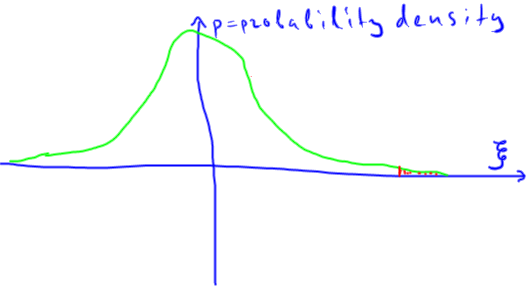
\includegraphics[scale=.5]{img/p-value.png}
    \caption{Площадь красного сегмента графика плотности вероятности случайной величины $\xi$ - это p-value, соответствующее значению $\xi$ на границе сегмента}
    \label{pval}
\end{figure}

\bibliographystyle{natbib}
\bibliography{p-values}

\end{document}
